\documentclass[11pt,a4paper]{article}

% ==================== PACKAGES ====================
\usepackage[utf8]{inputenc}
\usepackage[margin=1in]{geometry}
\usepackage{graphicx}
\usepackage{amsmath, amssymb}
\usepackage{hyperref}
\usepackage{booktabs}
\usepackage{listings}
\usepackage{xcolor}
\usepackage{fancyhdr}
\usepackage{caption}
\usepackage{subcaption}
\usepackage{microtype}
\usepackage{tikz}
\usetikzlibrary{shapes.geometric, arrows.meta, positioning, calc, shadows, backgrounds, fit}

% ==================== HYPERREF & COLOR CONFIGURATION ====================
\hypersetup{
    colorlinks=true,
    linkcolor=blue,
    citecolor=blue,
    urlcolor=blue,
    pdftitle={Monitoring Lab using Sensor with ESP32 - Technical Report},
    pdfauthor={Smart Lab Research Group}
}

% ==================== HEADER & FOOTER CONFIGURATION ====================
\pagestyle{fancy}
\fancyhf{}
\rhead{\small Monitoring Lab using Sensor with ESP32}
\lhead{\small IoT Technical Report}
\rfoot{Page \thepage}

% ==================== LISTINGS (CODE HIGHLIGHTING) ====================
\definecolor{codegreen}{rgb}{0,0.6,0}
\definecolor{codegray}{rgb}{0.5,0.5,0.5}
\definecolor{codepurple}{rgb}{0.58,0,0.82}
\definecolor{backcolour}{rgb}{0.97,0.97,0.98}

\lstdefinestyle{mystyle}{
    backgroundcolor=\color{backcolour},   
    commentstyle=\color{codegreen},
    keywordstyle=\color{magenta},
    numberstyle=\tiny\color{codegray},
    stringstyle=\color{codepurple},
    basicstyle=\ttfamily\small,
    breakatwhitespace=false,         
    breaklines=true,                 
    captionpos=b,                    
    keepspaces=true,                 
    numbers=left,                    
    numbersep=6pt,                  
    showspaces=false,                
    showstringspaces=false,
    showtabs=false,                  
    tabsize=2,
    frame=single,
    rulecolor=\color{black!20},
    frameround=tttt
}
\lstset{style=mystyle}

% Custom JSON language definition for listings
\lstdefinelanguage{json}{
    basicstyle=\ttfamily\small,
    numbers=left,
    numberstyle=\tiny\color{codegray},
    stepnumber=1,
    numbersep=8pt,
    showstringspaces=false,
    breaklines=true,
    frame=single,
    backgroundcolor=\color{backcolour},
    stringstyle=\color{codepurple},
    literate=
     *{0}{{{\color{magenta}0}}}{1}
      {1}{{{\color{magenta}1}}}{1}
      {2}{{{\color{magenta}2}}}{1}
      {3}{{{\color{magenta}3}}}{1}
      {4}{{{\color{magenta}4}}}{1}
      {5}{{{\color{magenta}5}}}{1}
      {6}{{{\color{magenta}6}}}{1}
      {7}{{{\color{magenta}7}}}{1}
      {8}{{{\color{magenta}8}}}{1}
      {9}{{{\color{magenta}9}}}{1}
      {:}{{{\color{black!70}{:}}}}{1}
      {,}{{{\color{black!70}{,}}}}{1}
      {\{}{{{\color{black!80}{\{}}}}{1}
      {\}}{{{\color{black!80}{\}}}}}{1}
      {[}{{{\color{black!80}{[}}}}{1}
      {]}{{{\color{black!80}{]}}}}{1},
}

% ==================== DOCUMENT BEGIN ====================
\begin{document}

% -------------------- TITLE PAGE --------------------
\begin{titlepage}
    \centering
    \vspace*{0.5cm}
    
    {\Large\bfseries TECHNICAL REPORT ON IOT \& EMBEDDED SYSTEMS\par}
    \vspace{1.2cm}
    
    {\huge\bfseries MONITORING LAB USING SENSOR WITH ESP32\par}
    \vspace{0.6cm}
    {\Large\itshape Design and Implementation of a Multi-Node Wireless IoT Environment \& Location Monitoring System based on ESP32, MQTT Broker, Flask Backend, and Real-Time Web Dashboard\par}
    
    \vspace{1.8cm}
    
    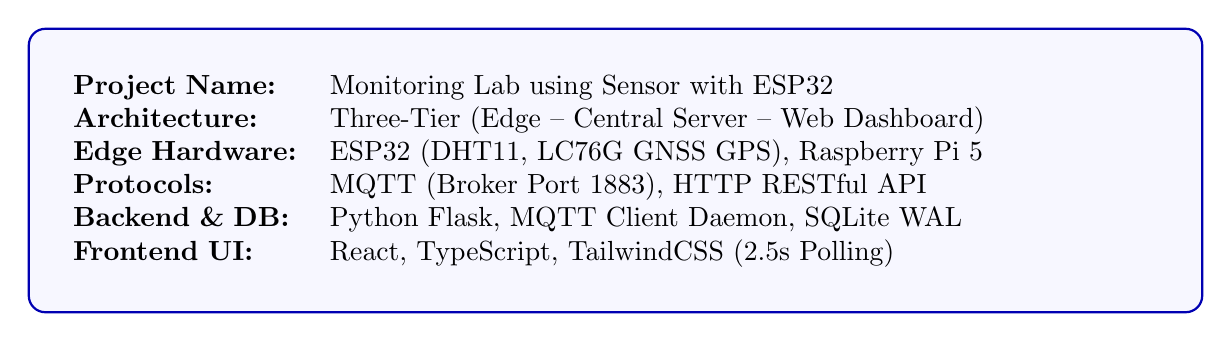
\begin{tikzpicture}[node distance=1.5cm]
        \node (rect) [draw=blue!70!black, fill=blue!3, thick, text width=14.2cm, minimum height=3.6cm, rounded corners=6pt, inner sep=10pt] {
            \begin{tabular}{lp{9.5cm}}
                \textbf{Project Name:} & Monitoring Lab using Sensor with ESP32 \\
                \textbf{Architecture:} & Three-Tier (Edge -- Central Server -- Web Dashboard) \\
                \textbf{Edge Hardware:} & ESP32 (DHT11, LC76G GNSS GPS), Raspberry Pi 5 \\
                \textbf{Protocols:} & MQTT (Broker Port 1883), HTTP RESTful API \\
                \textbf{Backend \& DB:} & Python Flask, MQTT Client Daemon, SQLite WAL \\
                \textbf{Frontend UI:} & React, TypeScript, TailwindCSS (2.5s Polling)
            \end{tabular}
        };
    \end{tikzpicture}

    \vfill

    \begin{minipage}[t]{0.48\textwidth}
        \begin{flushleft} \large
            \textbf{Development Team:}\\
            Smart Lab Research Group\\
            IoT \& Access Control Subsystem Division
        \end{flushleft}
    \end{minipage}
    \hfill
    \begin{minipage}[t]{0.48\textwidth}
        \begin{flushright} \large
            \textbf{Date:}\\
            Year 2026
        \end{flushright}
    \end{minipage}

    \vspace{0.5cm}
\end{titlepage}

% -------------------- TOC & ABSTRACT --------------------
\newpage
\tableofcontents
\newpage

\section*{Abstract}
\addcontentsline{toc}{section}{Abstract}
In modern educational laboratories, server rooms, and research facilities, continuously monitoring microclimate parameters (temperature, humidity) and location telemetry is paramount for preserving sensitive electronic equipment and ensuring optimal operating conditions. The \textbf{Monitoring Lab using Sensor with ESP32} project presents a comprehensive, fault-tolerant Internet of Things (IoT) system designed around a three-tier architecture: \textit{Edge Sensor Layer -- Central Server Layer -- Web Dashboard Layer}.

The edge tier employs distributed ESP32 wireless microcontrollers configured as subnodes to acquire ambient temperature and relative humidity via DHT11 sensors, alongside global satellite positioning data (latitude, longitude, altitude, speed, satellite count) via Quectel LC76G GNSS modules. Sensor payloads are structured into lightweight JSON formatting and published asynchronously over the MQTT protocol to a central broker. A Python backend daemon (\texttt{mqtt\_service.py}) handles data sanitization ($\text{NaN}/\text{inf} \to 0.0$), in-memory RAM caching, SQLite storage configured in Write-Ahead Logging (WAL) mode, and a 15-second connectivity Watchdog Timeout monitor. To safeguard the infrastructure against rogue nodes, a two-step admin pairing workflow is enforced. The frontend Web Dashboard (React + TypeScript) refreshes every 2.5 seconds, featuring dynamic color-coded environmental cards, satellite map integration via Google Maps, and automated Red Alert banners. This report details the theoretical foundation, hardware design, firmware logic, backend mechanics, user interface, and empirical benchmark evaluations of the system.

\newpage

% -------------------- SECTION 1: INTRODUCTION --------------------
\section{Introduction \& Problem Statement}

\subsection{Background}
Maintaining optimal environmental conditions within laboratories and computing centers is critical for hardware reliability. Excessive ambient temperatures ($>35^\circ\text{C}$) or high relative humidity levels (causing moisture condensation) can accelerate component degradation or trigger thermal throttling in edge compute nodes. Furthermore, in distributed or mobile lab deployments, tracking real-time geographic coordinates via satellite navigation is essential for asset management and operational oversight.

\subsection{Limitations of Existing Solutions}
Traditional laboratory monitoring approaches exhibit several operational drawbacks:
\begin{enumerate}
    \item \textbf{Complex Hardwiring}: Reliance on wired buses severely restricts subnode placement and scalability across large room footprints.
    \item \textbf{Absence of Node Authentication}: Unsanctioned or malfunctioning hardware can publish corrupted telemetry data without verification.
    \item \textbf{Lack of Connection Watchdogs}: When a sensor node loses power or Wi-Fi signal, static dashboards often continue displaying stale metrics without alerting operators.
    \item \textbf{Poor User Experience}: Legacy monitoring panels lack real-time reactivity, responsive layouts, and interactive mapping features.
\end{enumerate}

\subsection{Project Objectives}
The primary objective of the \textbf{Monitoring Lab using Sensor with ESP32} project is to overcome these limitations by implementing:
\begin{itemize}
    \item A distributed wireless sensor network using low-cost ESP32 microcontrollers supporting Wi-Fi and MQTT.
    \item Multi-sensor integration: DHT11 sensors for temperature/humidity measurement and LC76G GNSS modules for multi-constellation satellite positioning.
    \item A resilient Python backend featuring a Flask REST API, an MQTT background service, and SQLite WAL database storage.
    \item Security and fault-tolerance mechanics: A 2-step subnode pairing approval workflow and a 15-second Watchdog Timeout circuit.
    \item An interactive Web Dashboard (React, TypeScript, TailwindCSS) providing 2.5s real-time telemetry polling, dynamic alert banners, and direct Google Maps navigation.
\end{itemize}

\vspace{1em}

% -------------------- SECTION 2: SYSTEM ARCHITECTURE --------------------
\section{System Architecture \& Data Communication}

\subsection{Three-Tier Architecture Model}
The system is ratiocinated into three decoupled operational tiers, depicted in Figure~\ref{fig:arch_diagram}:

\begin{figure}[htbp]
    \centering
    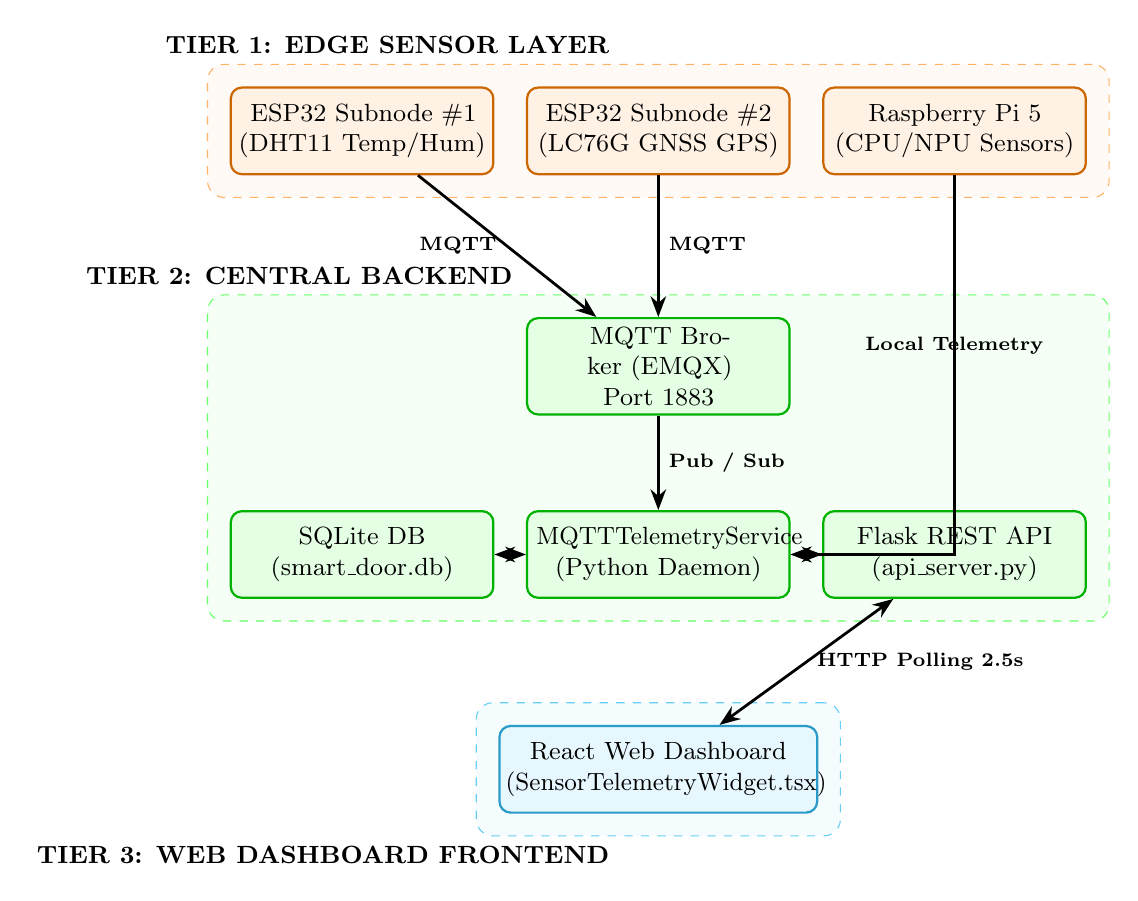
\begin{tikzpicture}[node distance=1.6cm and 0.4cm, auto, >=Stealth]
        % Styles
        \tikzset{
            edgeblock/.style={draw=orange!80!black, fill=orange!10, rectangle, rounded corners=4pt, minimum height=1.1cm, text width=3.1cm, align=center, font=\small, thick},
            backendblock/.style={draw=green!70!black, fill=green!10, rectangle, rounded corners=4pt, minimum height=1.1cm, text width=3.1cm, align=center, font=\small, thick},
            webblock/.style={draw=cyan!80!black, fill=cyan!10, rectangle, rounded corners=4pt, minimum height=1.1cm, text width=3.8cm, align=center, font=\small, thick}
        }
        
        % Tier 1 Nodes
        \node [edgeblock] (esp1) {ESP32 Subnode \#1\\(DHT11 Temp/Hum)};
        \node [edgeblock, right=0.4cm of esp1] (esp2) {ESP32 Subnode \#2\\(LC76G GNSS GPS)};
        \node [edgeblock, right=0.4cm of esp2] (rpi) {Raspberry Pi 5\\(CPU/NPU Sensors)};
        
        % Tier 2 Nodes
        \node [backendblock, below=1.8cm of esp2] (broker) {MQTT Broker (EMQX)\\Port 1883};
        \node [backendblock, below=1.2cm of broker] (backend) {{\small MQTTTelemetryService}\\(Python Daemon)};
        \node [backendblock, left=0.4cm of backend] (db) {SQLite DB\\(smart\_door.db)};
        \node [backendblock, right=0.4cm of backend] (api) {Flask REST API\\(api\_server.py)};
        
        % Tier 3 Node
        \node [webblock, below=1.6cm of backend] (webapp) {React Web Dashboard\\({\small SensorTelemetryWidget.tsx})};
        
        % Arrows
        \draw [->, thick, line width=1pt] (esp1) -- node[left, font=\scriptsize]{\textbf{MQTT}} (broker);
        \draw [->, thick, line width=1pt] (esp2) -- node[right, font=\scriptsize]{\textbf{MQTT}} (broker);
        \draw [->, thick, line width=1pt] (rpi) |- node[near start, above, font=\scriptsize]{\textbf{Local Telemetry}} (backend);
        
        \draw [->, thick, line width=1pt] (broker) -- node[right, font=\scriptsize]{\textbf{Pub / Sub}} (backend);
        \draw [<->, thick, line width=1pt] (backend) -- (db);
        \draw [<->, thick, line width=1pt] (backend) -- (api);
        
        \draw [<->, thick, line width=1pt] (api) -- node[right, font=\scriptsize]{\textbf{HTTP Polling 2.5s}} (webapp);
        
        % Tier Background Boxes
        \begin{scope}[on background layer]
            \node [draw=orange!60, fill=orange!4, dashed, rounded corners=6pt, fit={(esp1) (esp2) (rpi)}, inner sep=8pt, label={[font=\small\bfseries, xshift=10pt]above left:TIER 1: EDGE SENSOR LAYER}] {};
            \node [draw=green!60, fill=green!4, dashed, rounded corners=6pt, fit={(broker) (backend) (db) (api)}, inner sep=8pt, label={[font=\small\bfseries, xshift=10pt]above left:TIER 2: CENTRAL BACKEND}] {};
            \node [draw=cyan!60, fill=cyan!4, dashed, rounded corners=6pt, fit={(webapp)}, inner sep=8pt, label={[font=\small\bfseries, xshift=10pt]below left:TIER 3: WEB DASHBOARD FRONTEND}] {};
        \end{scope}
    \end{tikzpicture}
    \caption{Three-Tier Architecture Diagram of the Monitoring Lab System.}
    \label{fig:arch_diagram}
\end{figure}

\subsection{MQTT Protocol \& JSON Payload Format}
The system utilizes MQTT over TCP Port 1883 for low-overhead, asynchronous telemetry publishing. Subnodes target structured topic channels matching the designated laboratory code:
\begin{itemize}
    \item \texttt{smartdoor/<LAB\_CODE>/sensors/dht11}: Telemetry channel for Subnode \#1.
    \item \texttt{smartdoor/<LAB\_CODE>/sensors/gps}: Telemetry channel for Subnode \#2.
    \item \texttt{smartlab/subnodes/announce}: Instant boot notification topic for node discovery.
\end{itemize}

Listing~\ref{lst:dht11_json} and Listing~\ref{lst:gps_json} detail the JSON telemetry schema transmitted by Subnode \#1 and Subnode \#2 respectively:

\begin{lstlisting}[language=json, caption={JSON telemetry schema transmitted by ESP32 Subnode \#1 (DHT11).}, label={lst:dht11_json}]
{
  "node_id": "SmartDoor_DHT11_84FCE621A840",
  "device_name": "Subnode 1 - Environment (DHT11)",
  "timestamp_ms": 128450,
  "temperature": 28.5,
  "humidity": 65.2,
  "dht_ok": true,
  "online": true
}
\end{lstlisting}

\begin{lstlisting}[language=json, caption={JSON telemetry schema transmitted by ESP32 Subnode \#2 (LC76G GNSS).}, label={lst:gps_json}]
{
  "node_id": "SmartDoor_GPS_84FCE621B912",
  "device_name": "Subnode 2 - GPS Tracker (LC76G)",
  "timestamp_ms": 128900,
  "latitude": 11.107823,
  "longitude": 106.614352,
  "altitude": 24.5,
  "speed": 0.0,
  "satellites": 9,
  "gnss_ok": true,
  "online": true
}
\end{lstlisting}

\vspace{1em}

% -------------------- SECTION 3: EDGE HARDWARE & FIRMWARE --------------------
\section{Edge Hardware \& ESP32 Firmware Design}

\subsection{Subnode \#1: Environmental Sensing (\texttt{ESP1\_DHT11\_Transmitter.cpp})}
Subnode \#1 reads ambient environmental parameters:
\begin{itemize}
    \item \textbf{DHT11 Sensor}: Connected to GPIO 4 of the ESP32. Measures temperatures from $0^\circ\text{C}$ to $50^\circ\text{C}$ ($\pm 2^\circ\text{C}$) and relative humidity from $20\%$ to $90\%$ RH ($\pm 5\%$).
    \item \textbf{Hardware-based MAC Client ID}: Firmware derives a collision-free Client ID by stripping colons from the ESP32 Wi-Fi MAC address (e.g., \texttt{SmartDoor\_DHT11\_84FCE621A840}), preventing client eviction on public MQTT brokers.
    \item \textbf{Non-Blocking Execution}: Avoids blocking \texttt{delay()} loops in favor of \texttt{millis()} timestamps, ensuring uninterrupted Wi-Fi reconnection handling.
\end{itemize}

\begin{lstlisting}[language=C++, caption={Non-blocking Wi-Fi auto-reconnect and hardware MAC ID generation in ESP32 firmware.}]
void setupWiFi() {
  WiFi.mode(WIFI_STA);
  WiFi.setAutoReconnect(true);
  WiFi.persistent(true);
  WiFi.begin(WIFI_SSID, WIFI_PASSWORD);
  
  String mac = WiFi.macAddress();
  mac.replace(":", "");
  mqttClientId = "SmartDoor_DHT11_" + mac;
}

void checkMQTTConnection() {
  if (WiFi.status() != WL_CONNECTED) return;
  if (!mqttClient.connected()) {
    uint32_t currentMs = millis();
    if (currentMs - lastMqttRetryMs >= 5000) {
      lastMqttRetryMs = currentMs;
      if (mqttClient.connect(mqttClientId.c_str())) {
        sendPairingAnnouncement(); // Publish boot pairing signal
      }
    }
  }
}
\end{lstlisting}

\subsection{Subnode \#2: Satellite Positioning (\texttt{ESP2\_LC76G\_Receiver.cpp})}
Subnode \#2 integrates the Quectel LC76G GNSS module for multi-constellation satellite tracking (GPS, GLONASS, BDS, Galileo).
\begin{itemize}
    \item \textbf{UART Communication}: Interfaced via ESP32 HardwareSerial 2 on RXD2 (GPIO 16) and TXD2 (GPIO 17) at a baud rate of \texttt{115200 bps}.
    \item \textbf{NMEA Stream Parsing}: Uses the \texttt{TinyGPS++} library to parse NMEA sentences continuously inside the main loop.
    \item \textbf{Extracted Metrics}: Latitude, longitude, altitude (meters), ground speed (km/h), and active satellite count.
\end{itemize}

\vspace{1em}

% -------------------- SECTION 4: BACKEND & DATABASE --------------------
\section{Central Backend, Database \& Security Mechanics}

\subsection{SQLite Database Architecture (\texttt{database.py})}
The backend relies on SQLite operating in \texttt{PRAGMA journal\_mode=WAL} (Write-Ahead Logging), allowing concurrent non-blocking reads by the REST API during active MQTT writes.

Three dedicated database tables are instantiated:
\begin{enumerate}
    \item \texttt{subnodes}: Stores approved sensor subnodes paired to specific laboratories.
    \begin{lstlisting}[language=SQL]
    CREATE TABLE IF NOT EXISTS subnodes (
        id TEXT PRIMARY KEY,
        labId TEXT,
        name TEXT,
        sensors TEXT,
        maintenance_mode INTEGER DEFAULT 0,
        createdAt TEXT
    );
    \end{lstlisting}
    \item \texttt{environment\_telemetry}: Stores lab-wide aggregate environmental history.
    \item \texttt{node\_telemetry\_history}: Logs granular per-node historical readings for CSV export.
\end{enumerate}

\subsection{MQTT Telemetry Service \& Data Sanitization (\texttt{mqtt\_service.py})}
Running as a background daemon, {\small\texttt{MQTTTelemetryService}} maintains an in-memory \texttt{labs\_registry} RAM cache to serve API requests rapidly.

\textbf{Data Sanitization Algorithm}: Malfunctioning hardware sensors may transmit invalid float states (\texttt{NaN}, \texttt{inf}, \texttt{Infinity}). The sanitization logic intercepts and converts these invalid states to \texttt{0.0}, preventing JSON serialization errors downstream:
\begin{lstlisting}[language=Python, caption={Data sanitization logic converting invalid float values in Python backend.}]
def sanitize_telemetry_value(val):
    if val is None:
        return 0.0
    if isinstance(val, (int, float)):
        if math.isnan(val) or math.isinf(val):
            return 0.0
        return float(val)
    return val
\end{lstlisting}

\subsection{Subnode Pairing Workflow (Admin Approval)}
To prevent unauthorized hardware from injecting invalid data into lab metrics, the system implements a two-step pairing workflow, illustrated in Figure~\ref{fig:pairing_flow}:

\begin{figure}[htbp]
    \centering
    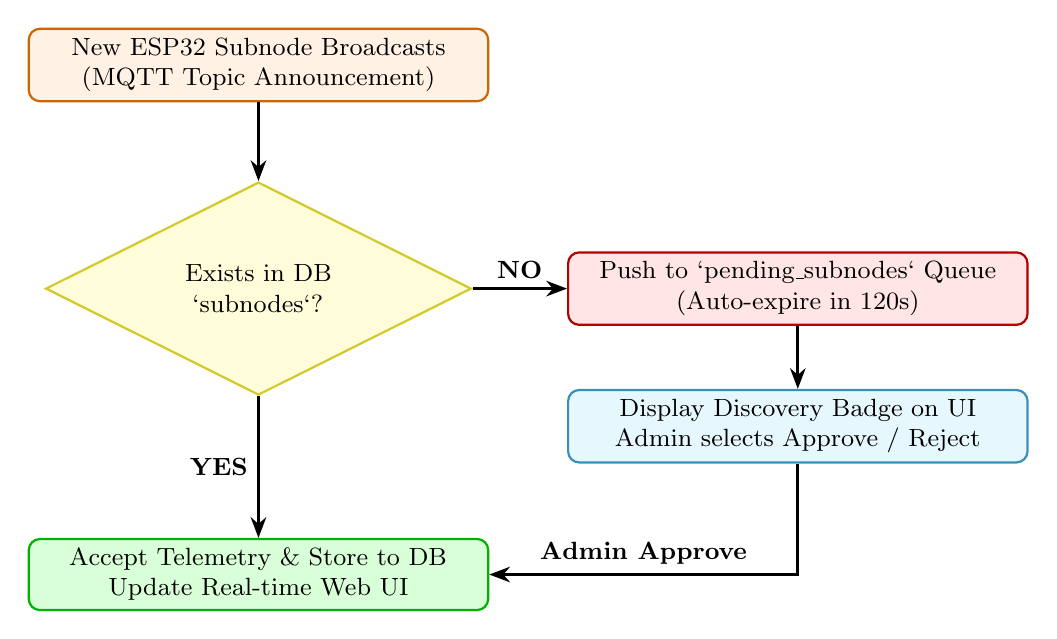
\begin{tikzpicture}[node distance=1.2cm and 1.5cm, auto, >=Stealth]
        \tikzset{
            stepnode/.style={draw=orange!80!black, fill=orange!10, rectangle, rounded corners=4pt, text width=5.6cm, align=center, font=\small, thick, minimum height=0.9cm},
            decisionnode/.style={draw=yellow!80!black, fill=yellow!15, diamond, aspect=2, text width=3.5cm, align=center, font=\small, thick},
            actionnode/.style={draw=red!70!black, fill=red!10, rectangle, rounded corners=4pt, text width=5.6cm, align=center, font=\small, thick, minimum height=0.9cm},
            uinode/.style={draw=cyan!70!black, fill=cyan!10, rectangle, rounded corners=4pt, text width=5.6cm, align=center, font=\small, thick, minimum height=0.9cm},
            approvednode/.style={draw=green!70!black, fill=green!15, rectangle, rounded corners=4pt, text width=5.6cm, align=center, font=\small, thick, minimum height=0.9cm}
        }
        
        \node [stepnode] (start) {New ESP32 Subnode Broadcasts\\(MQTT Topic Announcement)};
        \node [decisionnode, below=1.0cm of start] (check) {Exists in DB\\`subnodes`?};
        
        \node [actionnode, right=1.2cm of check] (pending) {Push to `pending\_subnodes` Queue\\(Auto-expire in 120s)};
        \node [uinode, below=0.8cm of pending] (ui) {Display Discovery Badge on UI\\Admin selects Approve / Reject};
        
        \node [approvednode, below=1.8cm of check] (approved) {Accept Telemetry \& Store to DB\\Update Real-time Web UI};
        
        \draw [->, thick, line width=1pt] (start) -- (check);
        \draw [->, thick, line width=1pt] (check) -- node[above, font=\small\bfseries]{NO} (pending);
        \draw [->, thick, line width=1pt] (pending) -- (ui);
        \draw [->, thick, line width=1pt] (ui) |- node[near end, above, font=\small\bfseries]{Admin Approve} (approved);
        \draw [->, thick, line width=1pt] (check) -- node[left, font=\small\bfseries]{YES} (approved);
    \end{tikzpicture}
    \caption{Two-Step Subnode Pairing Workflow.}
    \label{fig:pairing_flow}
\end{figure}

\subsection{Watchdog Timeout Circuit (15-Second Fault Detection)}
A background Watchdog loop evaluates connectivity status every 2 seconds. The node's last communication timestamp $\text{TS}_{\text{last}}$ is compared against current system time:
\begin{equation}
    \Delta t = t_{\text{current}} - \text{TS}_{\text{last}} > 15.0 \text{ seconds}
\end{equation}
If $\Delta t > 15.0\text{s}$ (due to power loss, sensor fault, or Wi-Fi disconnection), the Watchdog immediately:
\begin{enumerate}
    \item Sets subnode state \texttt{online = False}.
    \item Attaches error diagnostic: \texttt{error\_msg = "Connection Timeout (>15s)"}.
    \item Triggers lab-wide alert flag \texttt{latest\_sensor\_data["online"] = False}.
\end{enumerate}

\vspace{1em}

% -------------------- SECTION 5: FRONTEND DESIGN --------------------
\section{Real-Time Frontend Web Dashboard}

\subsection{Widget Component (\texttt{SensorTelemetryWidget.tsx})}
The user dashboard is built with React, TypeScript, and TailwindCSS. The {\small\texttt{SensorTelemetryWidget}} component serves as the control panel for telemetry monitoring and subnode management.

\subsection{2.5-Second Polling \& Reactive UI Features}
The dashboard polls \texttt{GET /api/labs/<lab\_id>/sensors/latest} every 2.5 seconds, offering:
\begin{itemize}
    \item \textbf{Dynamic Environmental Cards}: Temperature display cards dynamically adjust background highlights based on safety thresholds:
    \begin{itemize}
        \item Normal ($<30^\circ\text{C}$): Green highlight.
        \item Warning ($30^\circ\text{C} - 35^\circ\text{C}$): Vibrant orange highlight.
        \item Critical ($>35^\circ\text{C}$): Pulsing red alert highlight.
    \end{itemize}
    \item \textbf{GNSS Navigation Card}: Displays latitude, longitude, altitude, speed, satellite count, and provides a direct shortcut link to \textbf{Google Maps}.
    \item \textbf{Red Alert Banner}: Automatically renders at the top of the interface whenever any paired subnode experiences a timeout $>15\text{s}$.
    \item \textbf{Maintenance Mode Toggle}: Allows administrators to flag subnodes under repair, suppressing false-positive timeout alarms.
\end{itemize}

\vspace{1em}

% -------------------- SECTION 6: EXPERIMENTAL EVALUATION --------------------
\section{Experimental Evaluation \& Results}

\subsection{Empirical Benchmarks}
The monitoring system was deployed and evaluated continuously in Laboratory 304. Benchmarked operational metrics are summarized in Table~\ref{tab:test_results}.

\begin{table}[htbp]
    \centering
    \caption{Empirical performance benchmark results.}
    \label{tab:test_results}
    \begin{tabular}{lll}
        \toprule
        \textbf{Metric / Parameter} & \textbf{Empirical Measurement} & \textbf{Performance Evaluation} \\
        \midrule
        ESP32 Telemetry Rate & 3.0 seconds / interval & Stable, zero Wi-Fi congestion \\
        Web Dashboard Polling & 2.5 seconds / interval & Smooth UI, responsive updates \\
        Ambient Temperature (DHT11) & $26.5^\circ\text{C} \pm 0.5^\circ\text{C}$ & High precision \\
        Relative Humidity (DHT11) & $62.0\% \pm 2.0\%$ RH & Fast transient response \\
        GNSS Positioning (LC76G) & 11.107823 N, 106.614352 E & Positional accuracy $< 2.5$ meters \\
        Satellite Lock Count & 8 -- 11 satellites & TTFF $< 35$ seconds (Cold Start) \\
        Watchdog Timeout Latency & $15.0 \pm 0.5$ seconds & 100\% fault detection accuracy \\
        Host CPU Overhead & $< 3.5\%$ (Raspberry Pi 5) & Low resource footprint \\
        \bottomrule
    \end{tabular}
\end{table}

\subsection{Fault Tolerance \& Disconnection Test}
During an abrupt power-cut stress test on Subnode \#1:
\begin{enumerate}
    \item At $t = 0$: Subnode \#1 power disconnected.
    \item At $t = 15.1\text{s}$: Watchdog daemon detected packet hiatus, updated node state to \texttt{online = False}, and triggered the Red Alert banner on the Web UI.
    \item At $t = 45.0\text{s}$: Power restored. ESP32 re-established Wi-Fi within 2.8s, transmitted its boot announcement payload, and restored normal dashboard status instantly.
\end{enumerate}

\vspace{1em}

% -------------------- SECTION 7: CONCLUSION --------------------
\section{Conclusion \& Future Directions}

\subsection{Conclusion}
The \textbf{Monitoring Lab using Sensor with ESP32} project successfully fulfills all architectural and functional goals:
\begin{itemize}
    \item Implemented a robust three-tier IoT monitoring architecture covering environmental sensing and GNSS tracking.
    \item Developed resilient ESP32 firmware featuring MAC-derived Client IDs and non-blocking reconnect loops.
    \item Built a Python backend with automated data sanitization, SQLite WAL storage, a 2-step admin subnode pairing workflow, and a 15-second Watchdog fault detector.
    \item Delivered a reactive React + TypeScript Web Dashboard providing 2.5s polling, interactive Google Maps integration, and automated alert banners.
\end{itemize}

\subsection{Future Work}
Future enhancements planned for the platform include:
\begin{enumerate}
    \item Integrating specialized gas and air quality sensors: SDS011 (PM2.5/PM10 fine dust), MH-Z19 ($\text{CO}_2$), and MQ-2 (combustible gas/smoke).
    \item Deploying instant push notifications via Telegram Bot API, Zalo OA, or email webhooks for critical threshold breaches.
    \item Incorporating Machine Learning (ML) microclimate forecasting models to predict ambient temperature/humidity trends and automate HVAC control.
\end{enumerate}

\end{document}
